%----------------------------------------------------------------------------
%bb defines the bounding box for the pdf
%viewport defines the area of the pdf used
%in sidewaysfigure the last entry in bb moves the caption toward/away the pic
%in sidewaysfigure the second entry in bb moves the pic toward/away the caption
%----------------------------------------------------------------------------
\begin{figure}
\scalebox{0.8}[0.8]{
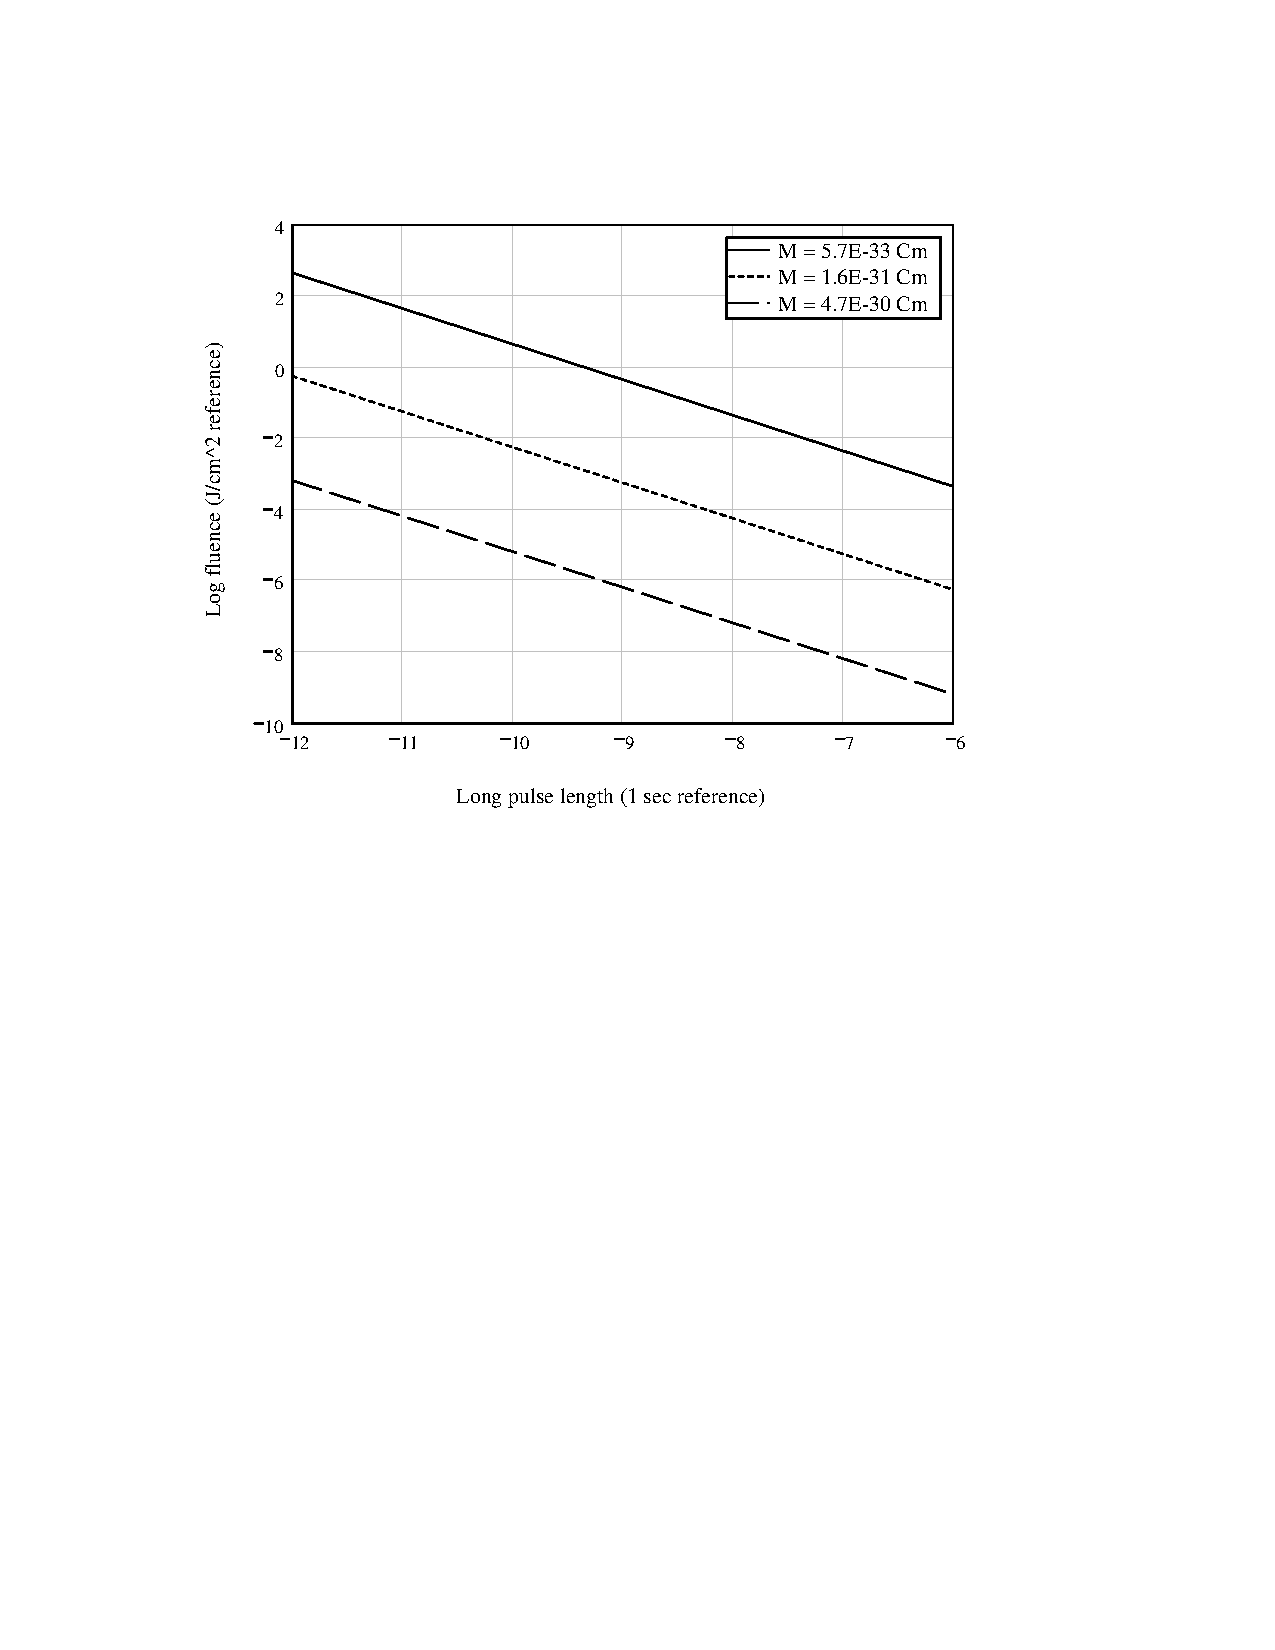
\includegraphics[bb=30 405 489 670]
{fluence/fluence.pdf}
}
\caption[Required fluence for inversion of the two level iodine molecule]{Required fluence for inversion of the two level iodine molecule. Here Equation \ref{required fluence} is plotted for various pulse lengths with $\Delta \tau = \pi/2$. To minimize the effect of collisions on the process, pulse length should be kept less that 1 ns when the target is at atmospheric pressure. A 1 ns pulse focused to a spot with a cross section area of about 1 mm$^2$ will need about 4 mJ to invert the two levels if we assume the ``weak'' coupling ($M=5.7\cross10^{-33}$ Cm). In an evacuated cell, one should be able to reduce the relaxiation effects to allow 100 ns pulses. In this case, the excitation beam (with the same 1 mm$^2$ cross section) must have over 0.7 mW of peak power, even when assuming ``strong'' coupling. ($M=4.7\cross10^{-30}$ Cm)}
\label{fluence}
\end{figure}
%----------------------------------------------------------------------------
